% Question figure contract — source physical pages in question-figure-map.json.
% Mode C; simple physics geometry, restrained blue/grey lines on white paper.
% Each question can be understood while hiding its solution. No solved labels.
% Reference geometry: preserve contacts, axis zero, directions, source point identities.
% Main viewport <=14cm; ordinary labels 9–11pt; all labels transparent.
% Read axes/objects first, givens second; no decoration or filled label rectangles.
% Cloned givens retain exact reviewed coordinates; answer overlays are excluded explicitly.
% Captions + source-specific labels bind each view to its own question, never previous answer.
% Anticipated risks: angle labels near rays, multiple dimensions, clipping tall multi-panels.
% Sketch: [question text] [given geometry or blank axes] -> [answer text + construction].

% Source example 2.1; question-only view.
\newcommand{\KQuestionAB}{%
\begin{center}\begin{minipage}{.97\linewidth}\centering
\begin{tikzpicture}[>=Latex,scale=.9]

\draw[kaxis] (-.25,0)--(6.6,0) node[right]{$t/\mathrm s$};
\draw[kaxis] (0,-2.7)--(0,1.2) node[above]{$x/\mathrm m$};
\foreach \t in {1,...,6}{\draw (\t,0)--(\t,.08);\node[above=2pt] at (\t,0){\t};}
\foreach \y/\v in {-2.4/-60,-1.6/-40,-.8/-20,.8/20}{\draw (0,\y)--(.08,\y);\node[left] at (0,\y){$\v$};}
\node[below left] at (0,0){$O$};

\end{tikzpicture}
\figcap{题图：按表中数据在空坐标系中作图。}\label{question-figure-2-1}
\end{minipage}\end{center}
}

% Source example 2.2; question-only view.
\newcommand{\KQuestionAC}{%
\begin{center}\begin{minipage}{.97\linewidth}\centering
\begin{tikzpicture}[>=Latex,scale=.85]

\foreach \dx/\i in {0/1,4.3/2,8.6/3}{\begin{scope}[xshift=\dx cm]
\draw[kaxis] (-.2,0)--(3.1,0) node[right]{$t$};
\draw[kaxis] (0,-.6)--(0,1.8) node[above]{$x$};
\node[below left] at (0,0){$O$};\node at (1.4,-.85){(\i)};
\end{scope}}

\end{tikzpicture}
\figcap{题图：分别画出三个运动函数的图像。}\label{question-figure-2-2}
\end{minipage}\end{center}
}

% Source example 2.3; question-only view.
\newcommand{\KQuestionAD}{%
\begin{center}\begin{minipage}{.97\linewidth}\centering
\begin{tikzpicture}[>=Latex,scale=.9]

\foreach \dx/\mode in {0/1,6.2/2}{\begin{scope}[xshift=\dx cm]
\draw[kaxis] (-.2,0)--(4.6,0) node[right]{$t$};
\draw[kaxis] (0,-1.25)--(0,1.3) node[above]{$x$};
\ifnum\mode=1
\draw[kcurve,domain=0:4.25,samples=200] plot(\x,{.8*sin(280*\x)});
\else
\draw[kcurve,domain=0:4.25,samples=240] plot(\x,{1.05*exp(-.85*\x)*cos(450*\x)});
\fi
\node[below left] at (0,0){$O$};\node at (2,-1.6){(\mode)};
\end{scope}}

\end{tikzpicture}
\figcap{题图：两个质点的一维位置随时间变化，坐标轴未给定数值比例。}\label{question-figure-2-3}
\end{minipage}\end{center}
}

% Source example 2.6; question-only view.
\newcommand{\KQuestionAG}{%
%
\begin{center}\begin{tikzpicture}[scale=.78,>=Latex]
  \foreach \dx/\mode in {-4.6/1,0/2,4.6/3}{
    \begin{scope}[xshift=\dx cm]
      \draw[kaxis] (-1.65,0)--(1.75,0) node[right,clearlabel]{$t$};
      \draw[kaxis] (-1.45,-.55)--(-1.45,2.05) node[above,clearlabel]{$x$};
      \ifnum\mode=1
        \draw[kcurve] (-1.35,0)--(0,1.35)--(1.35,0);
      \else\ifnum\mode=2
        \draw[kcurve,domain=-1.35:1.30,samples=80] plot (\x,{.25*(\x+1.35)^2});
      \else
        \draw[kcurve,domain=-1.35:1.35,samples=100] plot (\x,{1.45*sqrt(max(0,1-(\x/1.35)^2))});
      \fi\fi
    \end{scope}}
\end{tikzpicture}\figcap{题图：从左到右为三幅给定的位置—时间图像。}\label{question-figure-2-6}\end{center}
}

% Source example 2.7; question-only view.
\newcommand{\KQuestionAH}{%
%
\begin{center}\begin{tikzpicture}[scale=.9,>=Latex]
  \begin{scope}[shift={(-4.9,-1.1)}]
    \draw[kaxis] (0,0)--(2.75,0) node[right,clearlabel]{$t$};
    \draw[kaxis] (0,-1.55)--(0,1.85) node[above,clearlabel]{$v$};
    \draw[kcurve] (0,1.3)--(2.4,-1.3);
    \node[clearlabel,left] at (0,1.3){$v_0$};
    \node[clearlabel,left] at (0,-1.3){$-v_0$};
    \draw[kguide] (0,-1.3)--(2.4,-1.3);
    \node[clearlabel,below left] at (0,0){$O$};
    \node[clearlabel,above right=2pt] at (1.2,0){$T/2$};
    \node[clearlabel,above] at (2.4,0){$T$};
    \node[clearlabel,below] at (1.2,-1.7){已知速度图};
  \end{scope}
  \foreach \dx/\dy/\mode/\tag in {-.7/0/1/A,3.3/0/2/B,-.7/-3.3/3/C,3.3/-3.3/4/D}{
    \begin{scope}[shift={(\dx,\dy)}]
      \draw[kaxis] (0,0)--(2.7,0) node[right,clearlabel]{$t$};
      \draw[kaxis] (0,-.25)--(0,1.65) node[above,clearlabel]{$x$};
      \ifnum\mode=1
        \draw[kcurve] (0,0)--(1.2,1.15)--(2.4,0);
      \else\ifnum\mode=2
        \draw[kcurve,domain=0:1,samples=70]
          plot ({2.4*\x},{4.6*\x*(1-\x)});
      \else\ifnum\mode=3
        \draw[kcurve,domain=0:1,samples=70] plot ({2.4*\x},{1.15*(2*\x-\x*\x)});
      \else
        \draw[kcurve] (0,1.15)--(1.2,0)--(2.4,.85);
      \fi\fi\fi
      \node[clearlabel,below left] at (0,0){$O$};
      \node[clearlabel,below=3pt] at (1.2,0){$T/2$};
      \node[clearlabel,below=3pt] at (2.4,0){$T$};
      \node[clearlabel,below] at (1.2,-.65){$\tag$};
    \end{scope}}
\end{tikzpicture}\figcap{题图：左图给出速度随时间的变化，右侧 A—D 为待选的位置图像。}\label{question-figure-2-7}\end{center}
}

% Source example 2.8; question-only view.
\newcommand{\KQuestionAI}{%
%
\begin{center}\begin{tikzpicture}[scale=.78,>=Latex]
  \foreach \dx/\mode in {-4.4/1,0/2,4.4/3}{
    \begin{scope}[xshift=\dx cm]
      \draw[kaxis] (-1.55,0)--(1.75,0) node[right,clearlabel]{时间};
      \draw[kaxis] (-1.35,-.25)--(-1.35,1.85) node[above,clearlabel]{$v$};
      \ifnum\mode=1
        \draw[kcurve] (-1.25,0)--(1.25,1.35);
        \draw[kguide] (1.25,0)--(1.25,1.35);
        \draw[kguide] (-1.35,1.35)--(1.25,1.35);
        \node[clearlabel,left] at (-1.35,1.35){$v$};
      \else\ifnum\mode=2
        \draw[kcurve] (-1.25,.55)--(1.25,1.35);
        \draw[kguide] (1.25,0)--(1.25,1.35);
        \draw[kguide] (-1.35,.55)--(-1.25,.55) (-1.35,1.35)--(1.25,1.35);
        \node[clearlabel,left] at (-1.35,.55){$v_0$};
        \node[clearlabel,left] at (-1.35,1.35){$v_1$};
      \else
        \draw[kcurve] (-1.25,0)--(-.42,1.35)--(1.25,0);
        \draw[kguide] (-.42,0)--(-.42,1.35);
        \draw[kguide] (-1.35,1.35)--(-.42,1.35);
        \node[clearlabel,left] at (-1.35,1.35){$v_0$};
        \node[clearlabel,below] at (-.42,0){$t/3$};
      \fi\fi
      \node[clearlabel,below] at (1.25,0){$t$};
    \end{scope}}
\end{tikzpicture}\figcap{题图：三个运动过程的速度—时间图像，求相应时间内的路程。}\label{question-figure-2-8}\end{center}
}

% Source example 2.17; question-only view.
\newcommand{\KQuestionAR}{%
%
\begin{center}\begin{tikzpicture}[scale=.9,>=Latex]
  \draw[very thick] (-1.4,0)--(1.4,0);
  \node[point,label={[clearlabel]below right=3pt:$B$}] (B) at (0,0) {};
  \node[point,label={[clearlabel]left:$A$}] (A) at (0,3.2) {};
  \draw[<->,TextGray] (.8,0)--(.8,3.2) node[midway,clearlabel,right]{$h$};
  \draw[DeepBlue,very thick,->] (B)--(0,1.15) node[midway,clearlabel,left]{$v_0$};
  \draw[Blue,very thick,->] (A)--(0,2.45) node[midway,clearlabel,left]{$g$};
\end{tikzpicture}\figcap{题图：A 球从上方释放，B 球从下方以初速度 $v_0$ 竖直抛出，初始间距为 $h$。}\label{question-figure-2-17}\end{center}
}

% Source example 2.19; question-only view.
\newcommand{\KQuestionAT}{%
%
\begin{center}\begin{tikzpicture}[scale=.85,>=Latex]
  \draw[very thick] (-1.7,0)--(1.7,0);
  \fill (0,2.7) circle (.12);
  \fill (0,.12) circle (.12);
  \draw[kguide] (0,.27)--(0,2.55);
  \draw[<->,TextGray] (.88,0)--(.88,2.7)
    node[midway,clearlabel,right=2pt]{$H$};
  \draw[DeepBlue,very thick,->] (-.35,1.0)--(-.35,.25) node[midway,clearlabel,left]{$u$};
  \draw[Blue,very thick,->] (.35,.25)--(.35,1.0) node[midway,clearlabel,right]{$eu$};
\end{tikzpicture}\figcap{题图：初始高度为 $H$；一次碰撞前、后的速率分别用 $u$、$eu$ 表示。}\label{question-figure-2-19}\end{center}
}

% Source example 2.22; question-only view.
\newcommand{\KQuestionAW}{%
\begin{center}\begin{minipage}{.97\linewidth}\centering
\begin{tikzpicture}[>=Latex,scale=.70]

\foreach \x in {-4,-3,-2,-1,1,2,3,4,5}{\draw[RuleGray,thin] (\x,-5.5)--(\x,-.8) (\x,.1)--(\x,5);}
\foreach \y in {-5,-4,-3,-2,-1,1,2,3,4,5}{\draw[RuleGray,thin] (-4,\y)--(-1.05,\y) (.12,\y)--(5.5,\y);}
\draw[kaxis] (-4.2,0)--(5.8,0) node[right]{$x$};
\draw[kaxis] (0,-5.7)--(0,5.3) node[above]{$y$};
\foreach \x in {-3,-2,-1,1,2,3,4,5}\node[below=2pt] at (\x,0){$\x$};
\foreach \y in {-5,-4,-3,-2,-1,1,2,3,4}\node[left=2pt] at (0,\y){$\y$};
\node[above left=3pt] at (0,0){$O$};

\end{tikzpicture}
\figcap{题图：在直角坐标网格中标出题设各点。}\label{question-figure-2-22}
\end{minipage}\end{center}
}

% Source example 2.23; question-only view.
\newcommand{\KQuestionAX}{%
\begin{center}\begin{minipage}{.97\linewidth}\centering
\begin{tikzpicture}[>=Latex,scale=.9]

\draw[kaxis] (0,0)--(6,0) node[right]{$r$};
\foreach \r in {1,...,5}{\draw (\r,0)--(\r,.1);\node[below] at (\r,0){$\r$};}
\node[left] at (0,0){$O$};
\path[use as bounding box] (-.5,-1.4) rectangle (6.4,1.4);

\end{tikzpicture}
\figcap{题图：以向右射线为极轴，逆时针为正角方向。}\label{question-figure-2-23}
\end{minipage}\end{center}
}

% Source example 2.28; question-only view.
\newcommand{\KQuestionBC}{%
\begin{center}\begin{minipage}{.97\linewidth}\centering
\begin{tikzpicture}[>=Latex,scale=.9]

\coordinate (A) at (3,0);\coordinate (M) at (0,3);\coordinate (N) at (6,3);
\coordinate (B) at (1.125,3);\coordinate (H) at (3,3);
\draw[kguide] (M)--(N) (A)--(H) (A)--(B);
\node[point,label=below:$A$] at (A){};
\node[left] at (M){$M$};\node[right] at (N){$N$};
\draw[vector] (B)--++(1.1,0) node[midway,above]{$v$};
\draw[vector] (A)--++(0,1.7) node[midway,right]{$u$};
\node[below left] at (B){$B$};\node[above right] at (H){$H$};
\draw[TextGray] (A)++(90:.8) arc(90:122:.8);\node at (2.64,1.13){$\theta$};
\draw[<->] (3.7,0)--(3.7,3) node[midway,right]{$L$};

\end{tikzpicture}
\figcap{题图：潜艇 A 与航线 MN 的垂直距离为 $L$，$\theta$ 从航线法线量起。}\label{question-figure-2-28}
\end{minipage}\end{center}
}

% Source example 2.29; question-only view.
\newcommand{\KQuestionBD}{%
\begin{center}\begin{minipage}{.97\linewidth}\centering
\begin{tikzpicture}[>=Latex,scale=.9]

\coordinate (A) at (0,0);\coordinate (B) at (4,2);\coordinate (X) at (6,0);
\draw[kaxis] (A)--(X) node[right]{$X$};\draw[thick] (A)--(B) node[midway,above left]{$d$};
\draw[vector] (A)--(1.3,0) node[midway,below]{$v$};
\draw[vector] (B)--++(.5,-1.1) node[right]{$v_p$};
\draw (0.8,0) arc(0:26.565:.8);\node at (1.12,.3){$\theta$};
\node[point,label=below left:$A$] at (A){};\node[point,label=above:$B$] at (B){};

\end{tikzpicture}
\figcap{题图：球沿 AX 运动，队员从 B 开始奔跑；奔跑方向待选。}\label{question-figure-2-29}
\end{minipage}\end{center}
}

% Source example 2.30; question-only view.
\newcommand{\KQuestionBE}{%
%
\begin{center}\begin{tikzpicture}[scale=.82,>=Latex]
  \coordinate (P) at (-3.7,-.75);\coordinate (Q) at (2.25,-.75);\coordinate (R) at (-.3,2.25);
  \draw[very thick] (P)--(Q);
  \draw[kguide] (Q)--(R);
  \draw[vector] (-3.25,-.75)--(-1.8,-.75) node[midway,clearlabel,above]{$\vect v_1$};
  \draw[vector] (1.93,-.38)--(.95,.78) node[midway,clearlabel,right]{$\vect v_2$};
  \draw pic[draw=TextGray,->,angle radius=8mm,"$\alpha$"{clearlabel}] {angle=R--Q--P};
  \draw[<->,TextGray] (P)--(Q) node[midway,clearlabel,below=3pt]{$l$};
  \node[point,label={[clearlabel]left:$A,P$}] at (P) {};
  \node[point,label={[clearlabel]right:$B,Q$}] at (Q) {};
  \node[clearlabel,above] at (R){$R$};
\end{tikzpicture}\figcap{题图：A、B 初始位于 P、Q，分别沿 PQ、QR 匀速运动。}\label{question-figure-2-30}\end{center}
}

% Source example 2.31; question-only view.
\newcommand{\KQuestionBF}{%
%
\begin{center}\begin{minipage}{.96\linewidth}\centering
\begin{tikzpicture}[>=Latex]
 \coordinate (A) at (-2.8,2.3);\coordinate (C) at (.2,0);\coordinate (B) at (1.7,-1.9);
 \coordinate (U) at (.2,1.4);\coordinate (D) at (.2,-1.4);
 \draw[thick] (-3.5,0)--(3.6,0) node[right]{岸线};
 \draw[kguide] (A)--(-2.8,0) (B)--(1.7,0) (U)--(D);
 \draw[vector] (A)--(C) node[pos=.35,above right=2pt]{$v_1$};
 \draw[vector] (C)--(B) node[pos=.45,above right=2pt]{$v_2$};
 \draw pic[draw=TextGray,angle radius=7mm] {angle=U--C--A};
 \draw pic[draw=TextGray,angle radius=7mm] {angle=D--C--B};
 \node at (-.24,1.03){$\theta_1$};\node at (.55,-1.1){$\theta_2$};
 \draw[<->,TextGray] (-3.3,0)--(-3.3,2.3) node[midway,left]{$d_1$};
 \draw[<->,TextGray] (2.15,0)--(2.15,-1.9) node[midway,right]{$d_2$};
 \draw[<->,TextGray] (-2.8,-2.5)--(.2,-2.5) node[midway,below]{$x$};
 \draw[<->,TextGray] (.2,-2.5)--(1.7,-2.5) node[midway,below]{$L-x$};
 \node[point,label=above left:$A$] at (A){};\node[point,label=below right:$B$] at (B){};
 \node[point,label=above right:$C$] at (C){};
\node[below left=3pt] at (-3.5,0){$M$};\node[above left=6pt] at (3.6,0){$N$};
\end{tikzpicture}
\figcap{题图：A 在岸上、B 在水中，C 为待选择的入水点；两垂足间距为 $L$。}\label{question-figure-2-31}
\end{minipage}\end{center}
}

% Source example 2.32; question-only view.
\newcommand{\KQuestionBG}{%
%
\begin{center}\begin{minipage}{.95\linewidth}\centering
\begin{tikzpicture}[>=Latex]
 \draw[thick] (-.15,0)--(8.2,0);\draw[thick] (4,0)--(4,1.2);
 \draw[<->,TextGray] (4.25,0)--(4.25,1.2) node[midway,right=2pt]{$h$};
 \draw[kguide] (0,0)--(0,3) (6,0)--(6,.3);
 \draw[kcurve,->,domain=0:5.6,samples=90] plot(\x,{3-3*\x*\x/31.36});
 \draw[vector] (0,3)--(1.3,3) node[midway,above]{$v_0$};
 \draw[<->,TextGray] (-.5,0)--(-.5,3) node[midway,left]{$H$};
 \draw[<->,TextGray] (0,-.75)--(4,-.75) node[midway,below]{$L$};
 \draw[<->,TextGray] (4,-.75)--(6,-.75) node[midway,below]{$l$};
 \node[above left] at (0,3){$A$};\node[below=3pt] at (4,0){球网};\node[below=3pt] at (6,0){发球线};
\draw[thick] (8,-.12)--(8,.25);
\draw[<->,TextGray] (0,-1.4)--(8,-1.4) node[midway,below]{$2L$};
\node[above] at (8,.25){底线};
\end{tikzpicture}
\figcap{题图：A 为水平击球点；全场长 $2L$，球网到对方发球线的距离为 $l$。}\label{question-figure-2-32}
\end{minipage}\end{center}
}

% Source example 2.33; question-only view.
\newcommand{\KQuestionBH}{%
%
\begin{center}\begin{minipage}{.95\linewidth}\centering
\begin{tikzpicture}[>=Latex]
 \coordinate (A) at (0,2);\coordinate (B) at (4,0);\coordinate (V) at (5.1,-1.1);\coordinate (X) at (5.3,0);
 \draw[thick] (-.2,0)--(4.35,0);\draw[kguide] (A)--(0,0) (B)--(X);
 \draw[kcurve,dashed,domain=0:4,samples=80] plot(\x,{2-\x*\x/8});
 \draw[vector] (A)--(1.3,2) node[midway,above]{$\vect v_0$};
 \draw[vector] (B)--(V) node[right=4pt]{$\vect v$};
 \draw pic[draw=TextGray,angle radius=6mm] {angle=V--B--X};
 \node[right] at (4.7,-.21){$45^\circ$};
 \draw[<->,TextGray] (-.5,0)--(-.5,2) node[midway,left]{$h$};
 \node[point] at (A){};\node[point] at (B){};
\end{tikzpicture}
\figcap{题图：从高度 $h$ 水平抛出，落地速度与水平线成 $45^\circ$。}\label{question-figure-2-33}
\end{minipage}\end{center}
}

% Source example 2.34; question-only view.
\newcommand{\KQuestionBI}{%
%
\begin{center}\begin{minipage}{.95\linewidth}\centering
\begin{tikzpicture}[scale=.95,>=Latex]
 \coordinate (A) at (0,0);\coordinate (B) at (7.2,0);\coordinate (V) at (52:1.5);
 \draw[thick] (-.4,0)--(7.6,0);
 \draw[kcurve,->,domain=0:7.2,samples=100] plot(\x,{tan(52)*\x*(1-\x/7.2)});
 \draw[vector] (A)--(V) node[above left]{$v_0$};
 \draw pic[draw=TextGray,angle radius=7mm] {angle=B--A--V};\node at (.97,.39){$\theta$};
 \draw[<->,TextGray] (0,-.55)--(7.2,-.55) node[midway,below]{$S$};
\end{tikzpicture}
\figcap{题图：初速度为 $v_0$、仰角为 $\theta$，抛出点与落点等高。}\label{question-figure-2-34}
\end{minipage}\end{center}
}

% Source example 2.35; question-only view.
\newcommand{\KQuestionBJ}{%
%
\begin{center}\begin{minipage}{.96\linewidth}\centering
\begin{tikzpicture}[scale=.9,>=Latex]
 \coordinate (A) at (0,0);\coordinate (B) at (6.4,0);
 \draw[thick] (-.3,0)--(6.8,0);
 \foreach \ang in {22,68}{\draw[kcurve,dashed,domain=0:6.4,samples=100] plot(\x,{tan(\ang)*\x*(1-\x/6.4)});
 \draw[vector] (A)--(\ang:1.3);}
 \draw[TextGray] (.7,0) arc[start angle=0,end angle=22,radius=.7];
 \draw[TextGray] (1.1,0) arc[start angle=0,end angle=68,radius=1.1];
 \node at (1.39,.95){$\theta_1$};\node at (1.55,.22){$\theta_2$};
 \node[above] at (3.2,4){高弧线};\node[above] at (3.2,.7){低弧线};
 \node[below] at (3.2,-.4){$\theta_1+\theta_2=\pi/2$，两次初速率相同};
\end{tikzpicture}
\figcap{题图：两次初速率相同，两个抛射角互余。}\label{question-figure-2-35}
\end{minipage}\end{center}
}

% Source example 2.36; question-only view.
\newcommand{\KQuestionBK}{%
\begin{center}\begin{minipage}{.97\linewidth}\centering
\begin{tikzpicture}[>=Latex,scale=.9]

\draw[thick] (-.3,0)--(6,0) (5,0)--(5,1.7);
\draw[vector] (0,0)--(52:1.5) node[above left]{$v_0$};
\draw (.7,0) arc(0:52:.7);\node at (1.03,.4){$\theta$};
\node[below left] at (0,0){$A$};
\draw[<->] (0,-.55)--(5,-.55) node[midway,below]{$L$};
\draw[<->] (5.5,0)--(5.5,1.7) node[midway,right]{$H$};

\end{tikzpicture}
\figcap{题图：A 到障碍物的水平距离为 $L$，障碍物高 $H$。}\label{question-figure-2-36}
\end{minipage}\end{center}
}

% Source example 2.37; question-only view.
\newcommand{\KQuestionBL}{%
%
\begin{center}\begin{minipage}{.96\linewidth}\centering
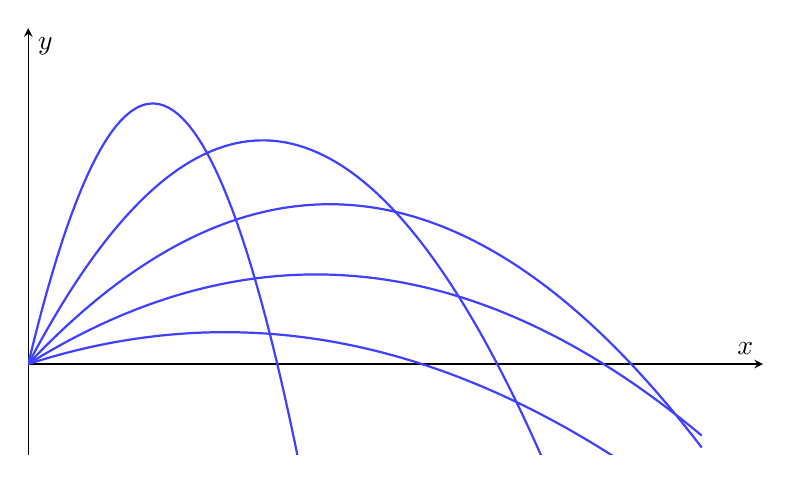
\begin{tikzpicture}
\begin{axis}[width=.90\linewidth,height=7cm,axis lines=middle,xlabel={$x$},ylabel={$y$},
 xmin=0,xmax=7.2,ymin=-1,ymax=3.7,ticks=none,clip=true]
 
 \foreach \ang in {20,35,50,65,78}{
  \addplot[Blue!75,thick,domain=0:6.6,samples=140]{x*tan(\ang)-x*x/(12*cos(\ang)^2)};
 }
\end{axis}
\end{tikzpicture}
\figcap{题图：从同一点以同一初速率、不同仰角抛出的轨迹族。}\label{question-figure-2-37}
\end{minipage}\end{center}
}

% Source example 2.39; question-only view.
\newcommand{\KQuestionBN}{%
%
\begin{center}\begin{minipage}{.96\linewidth}\centering
\begin{tikzpicture}[>=Latex]
 \coordinate (C) at (0,0);\coordinate (T) at (5,1.5);\coordinate (X) at (5.8,0);
 \draw[thick] (C)--(X) (C)--(5.6,1.68);
 \draw[kcurve,dashed,->,domain=0:5,samples=100] plot(\x,{tan(55)*\x-(5*tan(55)-1.5)*\x*\x/25});
 \draw[vector] (C)--(55:1.3) node[above left]{$v_0$};
 \draw[TextGray] (.75,0) arc[start angle=0,end angle={atan(.3)},radius=.75];
 \draw[TextGray] (1.3,0) arc[start angle=0,end angle=55,radius=1.3];
 \node at (.99,.10){$\alpha$};\node at (1.48,.75){$\beta$};
 \draw[kguide] (T)--(5,0);
 \draw[<->,TextGray] (0,-.55)--(5,-.55) node[midway,below]{$L$};
 \node[point,label=below left:$C$] at (C){};\node[point,label=above right:$T$] at (T){};
\end{tikzpicture}
\figcap{题图：坡脚 C、坡上目标 T；$\alpha$ 为坡角，$\beta$ 为发射仰角。}\label{question-figure-2-39}
\end{minipage}\end{center}
}

% Source example 2.40; question-only view.
\newcommand{\KQuestionBO}{%
%
\begin{center}\begin{minipage}{.96\linewidth}\centering
\begin{tikzpicture}[>=Latex]
 \draw[thick] (-.3,0)--(6.5,0) (5,0)--(5,2);
 \draw[kcurve,dashed,domain=0:5,samples=100] plot(\x,{2-2*(\x-5)^2/25});
 \draw[vector] (0,0)--({1.3/sqrt(1.64)},{1.04/sqrt(1.64)}) node[above left]{$v_0$};
 \draw[vector] (5,2)--(6.3,2) node[midway,above]{$v_T$};
 \draw[TextGray] (.7,0) arc[start angle=0,end angle={atan(.8)},radius=.7];
 \node at (1.02,.31){$\theta$};
 \draw[<->,TextGray] (0,-.55)--(5,-.55) node[midway,below]{$L$};
 \draw[<->,TextGray] (5.5,0)--(5.5,2) node[midway,right]{$H$};
 \node[below left] at (0,0){$A$};\node[above left] at (5,2){$T$};
\end{tikzpicture}
\figcap{题图：要求抛体在障碍顶端 T 处的速度平行于水平地面。}\label{question-figure-2-40}
\end{minipage}\end{center}
}

% Source example 2.41; question-only view.
\newcommand{\KQuestionBP}{%
%
\begin{center}\begin{minipage}{.96\linewidth}\centering
\begin{tikzpicture}[scale=.95,>=Latex]
 \pgfmathsetmacro{\thetaLaunch}{20+atan(1/(2*tan(20)))}
 \pgfmathsetmacro{\uu}{tan(\thetaLaunch)}
 \pgfmathsetmacro{\kk}{(\uu-tan(20))/4.5}
 \coordinate (A) at (0,0);\coordinate (P) at (4.5,{4.5*tan(20)});
 \coordinate (B) at (5.6,{5.6*tan(20)});\coordinate (V) at ($(P)+(-70:1.2)$);
 \draw[thick] (A)--(5.9,0) (A)--(B)--(5.6,0);
 \draw[kcurve,dashed,domain=0:4.5,samples=100] plot(\x,{\uu*\x-\kk*\x*\x});
 \draw[vector] (A)--(\thetaLaunch:1.3) node[above left]{$v_0$};
 \draw[vector] (P)--(V) node[right=3pt]{$v_P$};
 \draw pic[draw=TextGray,angle radius=4mm] {right angle=A--P--V};
 \draw[TextGray] (.7,0) arc[start angle=0,end angle=20,radius=.7];
 \draw[TextGray] (1.3,0) arc[start angle=0,end angle=\thetaLaunch,radius=1.3];
 \node at (.96,.14){$\alpha$};\node at (1.42,.9){$\theta$};
 \node[point,label=above right:$P$] at (P){};
\end{tikzpicture}
\figcap{题图：从斜面底端抛出，要求再次碰到斜面时速度垂直于斜面。}\label{question-figure-2-41}
\end{minipage}\end{center}
}

% Source example 2.43; question-only view.
\newcommand{\KQuestionBR}{%
%
\begin{center}\begin{minipage}{.98\linewidth}\centering
\begin{tikzpicture}[scale=1,>=Latex]
 \pgfmathsetmacro{\hh}{1/(1-.45^2)}\pgfmathsetmacro{\xa}{1.4-1.8/1.45}
 \draw[very thick] (-.1,3)--(2.3,3)--(2.3,2)--(4.1,2)--(4.1,1)--(5.9,1)--(5.9,0)--(7.8,0);
 \draw[kcurve,domain=0:1,samples=70] plot({\xa+(1.4-\xa)*\x},{3+\hh-\hh*\x*\x});
 \foreach \n in {0,1,2}{
  \draw[kcurve,domain=0:1,samples=90] plot({1.4+1.8*\n+1.8*\x},{3-\n+2*.45/(1-.45)*\x-(1+.45)/(1-.45)*\x*\x});
 }
 \foreach \n in {0,1,2,3}{\node[point,label=below:{$C_{\n}$}] at ({1.4+1.8*\n},{3-\n}){};}
 \draw[vector] (\xa,{3+\hh})--++(1.1,0) node[midway,above]{$v_0$};
 \node[above left] at (\xa,{3+\hh}){$A$};
 \draw[<->,TextGray] (-.45,3)--(-.45,{3+\hh}) node[midway,left]{$H$};
 \draw[<->,TextGray] (3.2,3.55)--(5,3.55) node[midway,above]{$d$};
 \draw[<->,TextGray] (7.4,0)--(7.4,1) node[midway,right]{$l$};
\end{tikzpicture}
\figcap{题图：A 在首个踏面上方 $H$；台阶宽 $d$、高 $l$，小球逐次反弹。}\label{question-figure-2-43}
\end{minipage}\end{center}
}

% Source example 2.45; question-only view.
\newcommand{\KQuestionBT}{%
\begin{center}\begin{minipage}{.97\linewidth}\centering
\begin{tikzpicture}[>=Latex,scale=.9]

\draw[thick] (-1.8,0)--(4.1,0);\draw[thick] (0,1.3) circle(1.3);
\coordinate (A) at (3.2,0);\coordinate (T) at (0,2.6);\coordinate (O) at (0,1.3);
\draw[kguide] (0,0)--(T);
\draw[kcurve,dashed,domain=0:3.2,samples=100] plot(\x,{2.6+.75*\x-(5/10.24)*\x*\x});
\pgfmathsetmacro{\launchangle}{180-atan(2.375)}
\draw[vector] (A)--++(\launchangle:1.3) node[above right]{$v_0$};
\draw[vector] (T)--++(-.8,-.6) node[above left]{$v_T$};
\draw[<->] (0,-.55)--(3.2,-.55) node[midway,below]{$d$};
\draw (O)--(-1.3,1.3) node[midway,above]{$R$};
\draw (A)++(\launchangle:.75) arc(\launchangle:180:.75);\node at (2.2,.38){$\theta$};
\node[point,label=below:$O$] at (O){};\node[point,label=above left:$T$] at (T){};
\node[point,label=below right:$A$] at (A){};

\end{tikzpicture}
\figcap{题图：A 为抛出点，T 为球顶；虚线仅示意一条可行轨迹，并非唯一轨迹。}\label{question-figure-2-45}
\end{minipage}\end{center}
}

% Source example 2.47; question-only view.
\newcommand{\KQuestionBV}{%
%
\begin{center}\RadialCollisionBase{\vect v_B}
\figcap{题图：A 沿半径为 $R$ 的圆周运动，B 沿 OP 匀速运动。}\label{question-figure-2-47}\end{center}
}

% Source example 2.48; question-only view.
\newcommand{\KQuestionBW}{%
%
\begin{center}\RadialCollisionBase{\vect a_B}
\figcap{题图：A 沿圆周匀速运动，B 从 O 由静止沿 OP 匀加速运动。}\label{question-figure-2-48}\end{center}
}

% Source example 2.49; question-only view.
\newcommand{\KQuestionBX}{%
%
\begin{center}\begin{tikzpicture}[scale=.8,>=Latex]
  \draw[very thick] (0,0) circle (2.25);
  \coordinate (O) at (0,0);\coordinate (P) at (90:2.25);\coordinate (Q) at (135:2.25);
  \draw[very thick] (O)--(P);\draw[kguide] (O)--(Q);
  \draw[DeepBlue,very thick,->] (125:2.5) arc[start angle=125,end angle=175,radius=2.5]
    node[midway,clearlabel,left]{$\omega_1$};
  \draw[Blue,very thick,->] (-2.5,-.55) arc[start angle=192,end angle=230,radius=2.5]
    node[midway,clearlabel,left]{$\omega_2$};
  \draw pic[draw=TextGray,->,angle radius=8mm,"$\theta$"{clearlabel}] {angle=P--O--Q};
  \node[point] at (Q) {};\node[left] at ($(Q)+(-.7,.32)$){$Q$};
  \node[point,label={[clearlabel]above:$P$}] at (P) {};
  \node[point,label={[clearlabel]below right:$O$}] at (O) {};
\end{tikzpicture}\figcap{题图：两质点从正上方 P 同时出发，逆时针运动；$\theta$ 标记再次相遇的位置。}\label{question-figure-2-49}\end{center}
}

% Source example 2.50; question-only view.
\newcommand{\KQuestionBY}{%
%
\begin{center}\begin{tikzpicture}[scale=.8,>=Latex]
  \draw[very thick] (0,0) circle (1.35);\draw[very thick] (0,0) circle (2.35);
  \coordinate (O) at (0,0);\coordinate (A) at (28:1.35);\coordinate (B) at (28:2.35);
  \draw[kguide] (O)--(B);
  \draw[vector] (A)--++(118:1.05) node[midway,clearlabel,right]{$\vect v_A$};
  \draw[vector] (B)--++(118:.82);
  \node at (2.12,2.17){$\vect v_B$};
  \draw[TextGray] (O)--(145:1.35) node[midway,clearlabel,above=3pt]{$R_1$};
  \draw[TextGray] (O)--(225:2.35);
  \node at (-1.75,-.65){$R_2$};
  \node[point] at (O) {};\node at (.25,-.30){$O$};
  \node[point,label={[clearlabel]right:$A$}] at (A) {};
  \node[point,label={[clearlabel]below right:$B$}] at (B) {};
\end{tikzpicture}\figcap{题图：A、B 分别在半径为 $R_1$、$R_2$ 的同心圆上同向运动。}\label{question-figure-2-50}\end{center}
}

% Source example 2.51; question-only view.
\newcommand{\KQuestionBZ}{%
%
\begin{center}\begin{minipage}{.96\linewidth}\centering
\begin{tikzpicture}[scale=1,>=Latex]
 \draw[TextGray,dashed] (3,0) arc[start angle=0,end angle=180,x radius=3,y radius=.75];
 \draw[thick] (-3,0) arc[start angle=180,end angle=360,x radius=3,y radius=.75];
 \coordinate (O) at (0,0);\coordinate (A) at (3,0);\coordinate (S) at (0,3);
 \draw[kguide] (O)--(A) (O)--(S);
 \draw[vector] (S)--(1.25,3) node[midway,above]{$v_0$};
 \draw[kcurve,dashed,->,domain=0:3,samples=90] plot(\x,{3-\x*\x/3});
 \draw[Blue,->,thick] (3.3,0) arc[start angle=0,end angle=52,x radius=3.3,y radius=.83];
 \node[above right] at (2.6,.7){$\omega$};
 \draw[<->,TextGray] (-.45,0)--(-.45,3) node[midway,left]{$H$};
 \node[below] at (1.5,0){$R$};
 \node[point,label=below left:$O$] at (O){};
 \node[point,label=right:$A$] at (A){};
 \node[point,label=above left:{$S\;(B\text{的初始位置})$}] at (S){};
\end{tikzpicture}
\figcap{题图：水平圆心 O 上方为 S；B 从 S 水平抛出，A 沿圆周运动。}\label{question-figure-2-51}
\end{minipage}\end{center}
}

% Source example 2.52; question-only view.
\newcommand{\KQuestionCA}{%
\begin{center}\begin{minipage}{.97\linewidth}\centering
\begin{tikzpicture}[>=Latex,scale=.9]

\draw[thick] (0,0) circle(1.5) (0,0) circle(2.6);
\coordinate (O) at (0,0);\coordinate (A) at (75:1.5);\coordinate (B) at (27:2.6);
\draw[kguide] (O)--(27:2.6) (O)--(A);\draw[thick] (A)--(B);
\pgfmathsetmacro{\lineangle}{atan2(1.5*sin(75)-2.6*sin(27),1.5*cos(75)-2.6*cos(27))}
\draw (B)++(\lineangle:.6) arc(\lineangle:207:.6);
\node at ($(B)+(190:.91)$){$\theta$};
\draw[->,DeepBlue] (80:1.78) arc(80:122:1.78) node[above left]{$\omega_1$};
\draw[->,DeepBlue] (5:2.87) arc(5:39:2.87) node[above right]{$\omega_2$};
\draw (O)--(150:1.5);\node at (-1.72,1.05){$R_1$};
\draw (O)--(230:2.6) node[pos=.7,below right]{$R_2$};
\node[point,label=below:$O$] at (O){};\node[point,label=above:$A$] at (A){};\node[point,label=right:$B$] at (B){};

\end{tikzpicture}
\figcap{题图：B 观察 A，视线 BA 与指向圆心的 BO 夹角为 $\theta$；图中未预设最大夹角位置。}\label{question-figure-2-52}
\end{minipage}\end{center}
}

% Source example 2.57; question-only view.
\newcommand{\KQuestionCF}{%
%
\begin{center}\begin{tikzpicture}[scale=.72,>=Latex]
 \draw[very thick] (-2.4,-2.4)--(-2.4,0) arc[start angle=180,end angle=0,radius=2.4]--(2.4,-2.4);
 \draw[very thick] (-1.4,-2.4)--(-1.4,0) arc[start angle=180,end angle=0,radius=1.4]--(1.4,-2.4);
 \draw[->,DeepBlue,very thick] (-1.4,-1.9)--(-1.4,-.85);
 \draw[->,Blue,very thick] (-2.4,-1.9)--(-2.4,-.85);
 \draw[<->,TextGray] (0,0)--(0,1.4) node[midway,clearlabel,right]{$R_1$};
 \draw[<->,TextGray] (0,0)--(135:2.4) node[pos=.85,clearlabel,above right=3pt]{$R_2$};
 \node[clearlabel,below] at (0,-2.75){内、外路线均为半圆弯道};
\end{tikzpicture}\figcap{题图：内、外半圆弯道半径分别为 $R_1,R_2$。}\label{question-figure-2-57}\end{center}
}

% Source example 2.59; question-only view.
\newcommand{\KQuestionCH}{%
%
\begin{center}\begin{minipage}{.96\linewidth}\centering
\begin{tikzpicture}[scale=.95,>=Latex]
 \draw[thick] (0,0) circle (2.0);\coordinate (P) at (35:2);
 \coordinate (V) at ($(P)+(125:1.4)$);\coordinate (A) at ($(P)+(170:1.4)$);
 \draw[kguide] (0,0)--(P) node[pos=.4,below right]{$R$};
 \draw[vector] (P)--(V) node[above right]{$\vect v$};
 \draw[vector] (P)--(A) node[above left]{$\vect a$};
 \draw pic[draw=TextGray,angle radius=7mm] {angle=V--P--A};
 % The circumference crosses this narrow wedge. Show its label separately,
 % retaining the physical vectors and the main angle arc without a mask.
 \begin{scope}[shift={(4.7,1.3)}]
 \draw[vector] (0,0)--(125:1.6) node[above right]{$\vect v$};
 \draw[vector] (0,0)--(170:1.6) node[above left]{$\vect a$};
 \draw[TextGray] (125:.6) arc(125:170:.6);
 \node at (147.5:.95){$\theta$};
 \node[below] at (-.5,-.4){夹角放大};
 \end{scope}
 \node[point,label=below left:$O$] at (0,0){};\node[point] at (P){};
\end{tikzpicture}
\figcap{题图：速度 $\vect v$ 与加速度 $\vect a$ 的夹角为 $\theta$。}\label{question-figure-2-59}
\end{minipage}\end{center}
}

% Source example 2.60; question-only view.
\newcommand{\KQuestionCI}{%
\begin{center}\begin{minipage}{.97\linewidth}\centering
\begin{tikzpicture}[>=Latex,scale=.9]

\draw[kaxis] (-3,0)--(3.2,0) node[right]{$x$};
\draw[kaxis] (0,-1.8)--(0,2) node[above]{$y$};\node[below left] at (0,0){$O$};

\end{tikzpicture}
\figcap{题图：根据给定参数方程在空坐标系中画出轨迹。}\label{question-figure-2-60}
\end{minipage}\end{center}
}

% Source example 2.61; question-only view.
\newcommand{\KQuestionCJ}{%
\begin{center}\begin{minipage}{.97\linewidth}\centering
\begin{tikzpicture}[>=Latex,scale=.9]

\draw[kaxis] (-3,0)--(3.2,0) node[right]{$x$};
\draw[kaxis] (0,-1.8)--(0,2) node[above]{$y$};\node[below left] at (0,0){$O$};

\end{tikzpicture}
\figcap{题图：根据给定参数方程在空坐标系中画出轨迹。}\label{question-figure-2-61}
\end{minipage}\end{center}
}

% Source example 2.62; question-only view.
\newcommand{\KQuestionCK}{%
%
\begin{center}\begin{tikzpicture}[scale=.72,>=Latex]
 \draw[very thick] (-.4,0)--(10,0);
 \draw[kaxis] (0,0)--(10.2,0) node[right,clearlabel]{$x$};\draw[kaxis] (0,0)--(0,3.4) node[above,clearlabel]{$y$};
 \draw[kcurve,domain=0:6.283,samples=120] plot ({1.35*(\x-sin(\x r))},{1.35*(1-cos(\x r))});
 \draw[very thick] (0,1.35) circle (1.35);\node[point,label={[clearlabel]below left:$P$}] at (0,0) {};
 \draw[vector] (0,1.35)--(1.1,1.35) node[pos=.22,clearlabel,above=3pt]{$v$};
\end{tikzpicture}\figcap{题图：圆沿水平地面无滑动滚动，P 为圆周上的标记点，初始位于接触处。}\label{question-figure-2-62}\end{center}
}

% Source example 2.63; question-only view.
\newcommand{\KQuestionCL}{%
\begin{center}\begin{minipage}{.97\linewidth}\centering
\begin{tikzpicture}[>=Latex,scale=.85,x={(1cm,0cm)},y={(-.50cm,-.28cm)},z={(0cm,.80cm)}]

\draw[kaxis] (0,0,0)--(3,0,0) node[right]{$x$};
\draw[kaxis] (0,0,0)--(0,2.8,0) node[below left]{$y$};
\draw[kaxis] (0,0,0)--(0,0,3.5) node[above]{$z$};
\node[below right] at (0,0,0){$O$};

\end{tikzpicture}
\figcap{题图：在右手直角坐标系中，根据三个坐标随时间的变化画出轨迹。}\label{question-figure-2-63}
\end{minipage}\end{center}
}

% Source example 2.64; question-only view.
\newcommand{\KQuestionCM}{%
%
\begin{center}\begin{tikzpicture}[scale=.78,>=Latex]
  \draw[kaxis] (-3.1,0)--(3.25,0) node[right,clearlabel]{$x$};
  \draw[kaxis] (0,-3.0)--(0,3.15) node[above,clearlabel]{$y$};
  \draw[very thick] (0,0) circle (2.25);
  \coordinate (O) at (0,0);\coordinate (P) at (38:2.25);
  \draw[very thick] (O)--(P) node[midway,clearlabel,below right]{$R$};
  \draw[kguide] (P)--(P|-O) node[clearlabel,below]{$x$};
  \draw[kguide] (P)--(P-|O) node[clearlabel,left]{$y$};
  \node[point,label={[clearlabel]below left:$O$}] at (O) {};
  \node[point,label={[clearlabel]above right:$P$}] at (P) {};
\end{tikzpicture}\figcap{题图：圆周上 P 点在两个坐标轴上的投影分别为 $x,y$。}\label{question-figure-2-64}\end{center}
}

% Source example 2.65; question-only view.
\newcommand{\KQuestionCN}{%
%
\begin{center}\begin{tikzpicture}[scale=.8,>=Latex]
  \draw[very thick] (-3.7,0)--(3.7,0);
  \draw[very thick] (0,1.55) circle (1.55);
  \coordinate (O) at (0,1.55);\coordinate (P) at (0,0);
  \draw[vector] (O)--++(1.45,0) node[midway,clearlabel,above]{$\vect v_O$};
  \draw[DeepBlue,very thick,->] ({1.85*cos(30)},{1.55+1.85*sin(30)}) arc[start angle=30,end angle=-20,radius=1.85];
  \node[clearlabel,right] at (2.05,1.15){$\omega$};
  \draw[very thick] (O)--(P) node[midway,clearlabel,right]{$R$};
  \node[point] at (P) {};\node[below=4pt] at (P){$P$};
  \node[point,label={[clearlabel]above left:$O$}] at (O) {};
\end{tikzpicture}\figcap{题图：圆无滑动向右滚动，P 为此刻与地面接触的圆周点。}\label{question-figure-2-65}\end{center}
}

% Source example 2.66; question-only view.
\newcommand{\KQuestionCO}{%
\begin{center}\begin{minipage}{.97\linewidth}\centering
\begin{tikzpicture}[>=Latex,scale=.9]

\draw[kaxis] (0,0)--(6,0) node[right]{$r$};\node[below left] at (0,0){$O$};
\path[use as bounding box] (-.5,-1.35) rectangle (6.4,1.35);

\end{tikzpicture}
\figcap{题图：以 O 为极点、向右为极轴，描出给定极坐标运动。}\label{question-figure-2-66}
\end{minipage}\end{center}
}

% Source example 2.68; question-only view.
\newcommand{\KQuestionCQ}{%
\begin{center}\begin{minipage}{.97\linewidth}\centering
\begin{tikzpicture}[>=Latex,scale=.9]

\draw[kaxis] (-2.2,0)--(2.3,0) node[right]{$x$};
\draw[kaxis] (0,-.7)--(0,2.7) node[above]{$y$};
\draw[kcurve,domain=-1.8:1.8,samples=100] plot(\x,{.65*\x*\x});
\node[below left] at (0,0){$O$};\node[right] at (1.8,2.1){$y=ax^2$};

\end{tikzpicture}
\figcap{题图：确定抛物线在原点处的曲率半径；这里示意 $a>0$。}\label{question-figure-2-68}
\end{minipage}\end{center}
}

% Source example 2.69; question-only view.
\newcommand{\KQuestionCR}{%
\begin{center}\begin{minipage}{.97\linewidth}\centering
\begin{tikzpicture}[>=Latex,scale=1.15]
\draw[kcurve] \FoldedCurvePath;\FoldedCurvePoints
\end{tikzpicture}
\figcap{题图：比较 $P_1,P_2,P_3,P_4$ 的局部弯曲，注意 $P_3$ 后向左下回折。}\label{question-figure-2-69}
\end{minipage}\end{center}
}

% Source example 2.70; question-only view.
\newcommand{\KQuestionCS}{%
\begin{center}\begin{minipage}{.97\linewidth}\centering
\begin{tikzpicture}[>=Latex,scale=.9]

\draw[thick] (0,0) ellipse(3 and 1.6);\draw (0,0)--(3,0) node[midway,below]{$a$};
\draw (0,0)--(0,1.6) node[midway,left]{$b$};\node[below left] at (0,0){$O$};

\end{tikzpicture}
\figcap{题图：椭圆的半长轴为 $a$、半短轴为 $b$。}\label{question-figure-2-70}
\end{minipage}\end{center}
}

% Source example 2.73; question-only view.
\newcommand{\KQuestionCV}{%
%
\begin{center}\begin{tikzpicture}[scale=.78,>=Latex]
 \fill[Blue!7] (-3,-1.45) rectangle (3,1.45);
 \draw[very thick] (-3,-1.45)--(3,-1.45) (-3,1.45)--(3,1.45);
 \coordinate (A) at (0,-1.45);\coordinate (B) at (0,1.45);
 \node[point,label={[clearlabel]below:$A$}] at (A) {};
 \node[point,label={[clearlabel]above:$B$}] at (B) {};
 \draw[vector] (-2.35,.15)--(-1.05,.15) node[midway,clearlabel,above]{$\vect u$};
 \draw[vector] (A)--++(145:1.25) node[near end,clearlabel,below left]{$\vect v$};
 \draw[<->,TextGray] (2.45,-1.45)--(2.45,1.45) node[midway,clearlabel,right]{$L$};
\end{tikzpicture}\figcap{题图：两岸正对的 A、B 距离为 $L$，水流速度向右，船速指船相对水的速度。}\label{question-figure-2-73}\end{center}
}

% Source example 2.74; question-only view.
\newcommand{\KQuestionCW}{%
%
\begin{center}\begin{tikzpicture}[scale=.82,>=Latex]
 \draw[very thick] (-3,0)--(3,0);
 \coordinate (A) at (-2.1,0);\coordinate (B) at (2.1,0);
 \node[point,label={[clearlabel]below:$A$}] at (A) {};
 \node[point,label={[clearlabel]below:$B$}] at (B) {};
 \draw[vector] (A)--++(1.55,0) node[midway,clearlabel,above]{$v$};
 \draw[vector] (-.75,1.0)--(.75,1.0) node[midway,clearlabel,above]{$S'\text{ 的速度 }u$};
\end{tikzpicture}\figcap{题图：地面系中 A 向右运动、B 静止；参考系 $S\prime$ 以速度 $u$ 向右平动。}\label{question-figure-2-74}\end{center}
}

% Source example 2.82; question-only view.
\newcommand{\KQuestionDE}{%
\begin{center}\begin{minipage}{.97\linewidth}\centering
\begin{tikzpicture}[>=Latex,scale=.9]

\draw[thick] (-2,0)--(3,0) (-2,2.7)--(3,2.7);
\node[point,label=below:$A$] at (0,0){};
\draw[vector] (-1.7,1.5)--(-.3,1.5) node[midway,above]{$v_2$};
\draw[vector] (0,0)--(110:1.4) node[pos=.5,right=7pt]{$v_1$};
\draw[<->] (2.4,0)--(2.4,2.7) node[midway,left]{$d$};

\end{tikzpicture}
\figcap{题图：水流平行于河岸，小船对水速度的大小为 $v_1$，船头方向可以选择。}\label{question-figure-2-82}
\end{minipage}\end{center}
}

% Source example 2.85; question-only view.
\newcommand{\KQuestionDH}{%
\begin{center}\begin{minipage}{.97\linewidth}\centering
\begin{tikzpicture}[>=Latex,scale=.9]

\coordinate (A) at (4,0);\coordinate (B) at (-2,2.4);\coordinate (C) at (2.4,2.4);
\draw[thick] (A)--(B) node[midway,below left]{$L$};
\draw[kguide] (B)--(5.1,2.4) (A)--(4,3.2) (A)--(C);
\draw[vector] (B)--(-.7,2.4) node[midway,above]{$v_1$};
\draw[vector] (A)--($(A)!.43!(C)$) node[left]{$v_2$};
\draw (B)++(-21.801:.85) arc(-21.801:0:.85);\node at (-.7,2.1){$\alpha$};
\draw (A)++(123.690:.65) arc(123.690:158.199:.65);\node at (3.23,.69){$\beta$};
\foreach \p/\pos in {A/below right,B/above left,C/above}\node[point,label=\pos:$\p$] at (\p){};

\end{tikzpicture}
\figcap{题图：A 为潜艇、B 为敌船初始位置，C 表示可能的相遇点；发射方向待定。}\label{question-figure-2-85}
\end{minipage}\end{center}
}

% Source example 2.87; question-only view.
\newcommand{\KQuestionDJ}{%
\begin{center}\begin{minipage}{.97\linewidth}\centering
\begin{tikzpicture}[>=Latex,scale=.9]

\draw[kguide] (0,0)--(4.8,0);
\foreach \x/\lab in {0/A,1.8/B,3.6/C}{\fill (\x,0) circle(1.5pt);\node[below] at (\x,0){$\lab$};}
\draw[vector] (0,0)--(.6,0);\node[above] at (.3,0){$u$};
\draw[vector] (1.8,0)--(1.8,1.2) node[above]{$2u$};
\draw[vector] (3.6,0)--(4.8,1.2) node[above]{$2\sqrt2u$};
\draw[<->] (0,-.65)--(1.8,-.65) node[midway,below]{$a$};
\draw[<->] (1.8,-.65)--(3.6,-.65) node[midway,below]{$a$};
\end{tikzpicture}
\figcap{题图：三船初始位置及对地速度，图中 A、B、C 等间距。}\label{question-figure-2-87}
\end{minipage}\end{center}
}

% Source example 2.89; question-only view.
\newcommand{\KQuestionDL}{%
\begin{center}\begin{minipage}{.97\linewidth}\centering
\begin{tikzpicture}[>=Latex,scale=.9]

\coordinate (O) at (0,0);\coordinate (A) at (0,3.6);\coordinate (B) at (4,0);\coordinate (P) at (1.52,2.232);
\draw[thick] (0,4.1)--(O)--(4.9,0);\draw[kcurve] (A)--(B);
\foreach \p/\pos in {A/left,B/below,P/above right}{\fill (\p) circle(1.5pt);\node[\pos] at (\p){$\p$};}
\draw[vector] (A)--++(0,-.8) node[midway,left]{$v_A$};\draw[vector] (B)--++(.8,0) node[above]{$v_B$};
\draw (0,2.9) arc(-90:-41.987:.7);\node at (.42,2.7){$\theta$};
\node[above right] at (.75,3.25){$aL$};\node[above right] at (2.7,1.4){$(1-a)L$};
\end{tikzpicture}
\figcap{题图：杆的 A、B 端接触墙、地；$\theta$ 从竖直墙量起，$AP=aL$。}\label{question-figure-2-89}
\end{minipage}\end{center}
}

% Source example 2.90; question-only view.
\newcommand{\KQuestionDM}{%
%
\begin{center}\begin{minipage}{\linewidth}\centering\begin{tikzpicture}[>=Latex,scale=.93]
\coordinate (O) at (0,2.5);\coordinate (B) at (4,0);
\draw[thick] (-3.8,2.3)--(-.15,2.3)--(-.15,-.4);
\fill[Blue!5] (0,-.7) rectangle (5.3,0);\draw[thin,Blue] (0,0)--(5.3,0);
\draw[thick] (-3.2,2.5) rectangle (-2.2,3);\draw (-3,2.4) circle(.1) (-2.4,2.4) circle(.1);
\draw[kcurve] (-2.2,2.5)--(O)--(B);
\fill (O) circle(1.8pt);\node[above right] at (O){$O$};
\draw[thick] (B)--(5.1,0)--(4.9,-.4)--(4.2,-.4)--cycle;
\fill (B) circle(1.5pt);\node[above right] at (B){$B$};
\draw[vector] (-2.3,3.45)--(-3.4,3.45) node[midway,above]{$v$};
\draw[vector] (4.9,-1)--(3.9,-1) node[midway,below]{$u$};
\node[above] at (-1.2,2.5){$l_c$};\node[above right] at (1.9,1.32){$l$};
\draw[<->] (-4.25,0)--(-4.25,2.5) node[midway,left]{$h$};
\draw[kguide] (-4.25,0)--(0,0) (-4.25,2.5)--(-3.5,2.5);
\draw (B)++(148:.9) arc(148:180:.9);\node at (2.82,.31){$\theta$};
\draw[<->] (0,-.85)--(4,-.85) node[midway,below]{$x$};
\end{tikzpicture}\figcap{题图：汽车经岸上定滑轮拉船；绳不可伸长，$h$ 为滑轮相对水面的高度。}\label{question-figure-2-90}\end{minipage}\end{center}
}

% Source example 2.91; question-only view.
\newcommand{\KQuestionDN}{%
\begin{center}\begin{minipage}{.97\linewidth}\centering
\begin{tikzpicture}[>=Latex,scale=.9]

\draw[thick] (0,0)--(4,0)--(0,2)--cycle;
\coordinate (P) at (2.2,.9);\draw[very thick] (P)--(2.2,3.1);
\foreach \x in {2.06,2.34}{\draw[thick] (\x,2)--(\x,2.6);}
\draw (1.6,2)--(2.06,2) (2.34,2)--(2.8,2);
\fill (P) circle(1.5pt);\node[above right=3pt] at (P){$P$};
\draw[vector] (.6,-.5)--(1.7,-.5) node[midway,below]{$v_0$};
\draw[vector] (2.7,2.65)--(2.7,3.5) node[right]{$v$};
\draw (3.2,0) arc(180:153.435:.8);\node at (2.95,.24){$\theta$};
\end{tikzpicture}
\figcap{题图：斜面向右运动，竖杆位于两侧固定导向之间，杆底 P 与斜面保持接触。}\label{question-figure-2-91}
\end{minipage}\end{center}
}

% Source example 2.92; question-only view.
\newcommand{\KQuestionDO}{%
\begin{center}\begin{minipage}{.97\linewidth}\centering
\begin{tikzpicture}[>=Latex,scale=.9]

\coordinate (C) at (0,0);\coordinate (P) at (1.2,1.6);
\draw[thick] (-2,0)--(2,0) arc(0:180:2);
\draw[kguide] (C)--(0,2.2) (C)--(P) (P)--(1.2,0);
\draw[very thick] (P)--(1.2,3.2);
\foreach \x in {1.06,1.34}{\draw[thick] (\x,2.4)--(\x,3);}
\draw (.6,2.4)--(1.06,2.4) (1.34,2.4)--(1.8,2.4);
\fill (P) circle(1.5pt) (C) circle(1.5pt);
\node[below left] at (C){$C=(X,0)$};\node[above right=3pt] at (P){$P$};
\node at (.7,.46){$R$};\node[below] at (1.2,0){$x_0$};
\draw (0,.75) arc(90:53.1301:.75);\node at (.29,1.13){$\theta$};
\draw[vector] (.5,-.8)--(1.6,-.8) node[midway,below]{$v_0$};
\end{tikzpicture}
\figcap{题图：半圆柱向右运动；竖杆横坐标固定，P 为接触点，$\theta$ 从竖直方向量起。}\label{question-figure-2-92}
\end{minipage}\end{center}
}

% Source example 2.93; question-only view.
\newcommand{\KQuestionDP}{%
%
\begin{center}\begin{minipage}{\linewidth}\centering\begin{tikzpicture}[>=Latex,scale=1]
\coordinate (O) at (0,0);\coordinate (B) at (0,3.4);\coordinate (A) at (2.3,1.2);\coordinate (C) at (-2.2,3.4);
\draw[very thick] (O)--(A) node[midway,below=5pt]{$R$};
\draw[kcurve] (A)--(B)--(C)--(-2.2,.65);
\draw[thick] (-2.55,0) rectangle (-1.85,.65);\node at (-2.2,.32){$M$};
\draw[kguide] (O)--(B);
\foreach \p/\pos in {O/below,B/above,C/above,A/right}{\fill (\p) circle(1.7pt);\node[\pos] at (\p){$\p$};}
\draw[<->] (-.65,0)--(-.65,3.4) node[midway,left]{$H$};
\draw (B)++(-90:.8) arc(-90:-43.727:.8);\node at (.42,2.4){$\alpha$};
\draw[->,DeepBlue] (35:.75) arc(35:120:.75);\node[above] at (.3,1.2){$\omega$};
\node[left] at (.83,2.0){$l$};
\end{tikzpicture}\figcap{题图：杆 OA 绕 O 转动，绳从 A 经固定转向点 B、C 连到物块 M。}\label{question-figure-2-93}\end{minipage}\end{center}
}

% Source example 2.94; question-only view.
\newcommand{\KQuestionDQ}{%
\begin{center}\begin{minipage}{.97\linewidth}\centering
\begin{tikzpicture}[>=Latex,scale=.9]

\draw[thick] (0,0)--(4,0);\node[point,label=left:$A$] at (0,0){};\node[point,label=right:$B$] at (4,0){};
\draw[vector] (0,0)--(0,1.6) node[above]{$v_A$};\draw[vector] (4,0)--(4,1.6) node[above]{$v_B$};
\draw[<->] (0,-.55)--(4,-.55) node[midway,below]{$l$};

\end{tikzpicture}
\figcap{题图：A、B 用轻杆连接；图示规定竖直向上为端点速度的正方向，各问按给定符号取向。}\label{question-figure-2-94}
\end{minipage}\end{center}
}

% Source example 2.95; question-only view.
\newcommand{\KQuestionDR}{%
%
\begin{center}\begin{minipage}{\linewidth}\centering\begin{tikzpicture}[>=Latex,scale=1]
\draw[thick] (-2,0)--(4,0);\draw[thick] (0,1) circle(1);
\fill (0,1) circle(1.5pt) (0,0) circle(1.5pt);\node[below left] at (0,1){$C$};\node[below left] at (0,0){$P$};
\draw (0,1)--(-.707,1.707);\node[left] at (-.58,1.28){$R$};
\draw[vector] (0,1)--(2.6,1);\node[above] at (2,1){$v_0$};
\draw[->,DeepBlue,thick] (40:1.5)++(0,1) arc(40:145:1.5);
\node[above] at (0,2.65){$\omega_0>0$（逆时针）};
\end{tikzpicture}\figcap{题图：球初始向右平动并逆时针转动，地面为水平面。}\label{question-figure-2-95}\end{minipage}\end{center}
}

% Source example 2.96; question-only view.
\newcommand{\KQuestionDS}{%
%
\begin{center}\begin{minipage}{\linewidth}\centering\begin{tikzpicture}[>=Latex]
\begin{scope}[x=2.1cm,y=2.1cm]
\draw[thick] (5,-.1)--(5,1.1);\node[right] at (5,.7){木靶};
\draw[kguide,domain=0:1,samples=100,variable=\t] plot({4.9*\t},{4.9*tan(30)*\t*(1-\t)});
\foreach \t/\n in {0/1,.25/2,.5/3,.75/4,1/5}{
\begin{scope}[shift={({4.9*\t},{4.9*tan(30)*\t*(1-\t)})},rotate={60+300*\t}]
\KnifeOutline\fill (0,0) circle(.7pt);
\end{scope}
\node[above] at ({4.9*\t},{4.9*tan(30)*\t*(1-\t)+.17}){\n};}
\draw[<->] (0,-.35)--(5,-.35) node[midway,below]{$s=5.0\,\mathrm m$};
\node at (2.5,-.8){(a) 质心抛物线与五个等时姿态};
\end{scope}
\begin{scope}[xshift=2.1cm,yshift=-3.8cm]
\begin{scope}[scale=15]\KnifeOutline\end{scope}
\fill (0,0) circle(1.5pt);\node[below] at (0,-.25){$C$};\node[right] at (1.5,0){刀尖};
\draw[<->] (-2.25,-.65)--(1.5,-.65) node[midway,below]{$L=25\,\mathrm{cm}$};
\draw[<->] (0,.65)--(1.5,.65) node[midway,above]{$l=10\,\mathrm{cm}$};
\node at (0,-1.45){(b) 长度定义（局部放大）};
\end{scope}
\begin{scope}[xshift=8cm,yshift=-3.8cm]
\draw[kaxis] (-.3,0)--(2.5,0) node[right]{$x$};
\begin{scope}[rotate=60,scale=10]\KnifeOutline\end{scope}
\draw[vector] (0,0)--(30:2.1) node[above right]{$\vect v_C$};
\draw (.65,0) arc(0:30:.65);\node at (15:.95){$30^\circ$};
\node[right] at (.25,-.45){$C$};\draw[thin] (.25,-.45)--(0,0);
\node[above] at (60:2.05){$\theta=60^\circ$};
\node at (.3,-2.45){(c) 初姿态与速度方向};
\end{scope}
\end{tikzpicture}\figcap{题图：飞刀的飞行姿态、长度及初始方向；木靶与初始质心等高。}\label{question-figure-2-96}\end{minipage}\end{center}
}

% Source example 2.103; question-only view.
\newcommand{\KQuestionDZ}{%
\begin{center}\begin{minipage}{.97\linewidth}\centering
\begin{tikzpicture}[>=Latex,scale=.9]

\coordinate (E) at (0,0);\coordinate (P) at (0,3.3);
\draw[thick] (E)--(P) node[midway,right]{$L$};
\draw (E) circle(.25);\node[below] at (0,-.3){地球 E};
\draw[vector] (P)--++(-135:1.5) node[below left]{$v$};
\draw (P)++(-135:.7) arc(-135:-90:.7);\node at (-.4,2.34){$\theta$};
\node[point,label=above:$P$] at (P){};

\end{tikzpicture}
\figcap{题图：天体初始距地球 $L$，运动方向与指向地球的视线成角 $\theta$。}\label{question-figure-2-103}
\end{minipage}\end{center}
}

% Source example 2.105; question-only view.
\newcommand{\KQuestionEB}{%
%
\begin{center}\begin{minipage}{\linewidth}\centering\begin{tikzpicture}[>=Latex,scale=.9]
\foreach \t/\n/\dx/\dy in {-90/1/0/0,-60/2/3.5/0,-36.37/3/7/0,0/4/10.5/0,36.37/5/1.75/-4,60/6/5.25/-4,90/7/8.75/-4}{
\begin{scope}[shift={(\dx,\dy)}]
\draw[TextGray] (0,0) circle(.8);\draw[thick] (0,0) circle({.8*1.524});
\fill (0,0) circle(1.3pt);\node[above] at (0,0){$S$};
\pgfmathsetmacro{\ea}{.985609*\t-90}
\pgfmathsetmacro{\ma}{.985609*\t*pow(1.524,-1.5)-90}
\pgfmathsetmacro{\ex}{.8*cos(\ea)}\pgfmathsetmacro{\ey}{.8*sin(\ea)}
\pgfmathsetmacro{\mx}{.8*1.524*cos(\ma)}\pgfmathsetmacro{\my}{.8*1.524*sin(\ma)}
\draw[DeepBlue,dashed,thin,->] (\ex,\ey)--({\ex+1.7*(\mx-\ex)},{\ey+1.7*(\my-\ey)});
\fill (\ex,\ey) circle(1.5pt) (\mx,\my) circle(1.5pt);
\node[font=\scriptsize] at (\ea:.5){$E_{\n}$};
\ifdim\t pt<0pt \node[font=\scriptsize,left] at ({\mx-.13},{\my-.16}){$M_{\n}$};
\else \node[font=\scriptsize,right] at ({\mx+.13},{\my-.16}){$M_{\n}$};\fi
\node[font=\footnotesize] at (0,1.7){\n：$t=\t\,\mathrm d$};
\end{scope}}
\node at (5.25,-6){虚线由地球经过火星，指向背景星空；各小图比例相同};
\end{tikzpicture}\figcap{题图：七个时刻的日、地、火位置与观测视线；E 为地球、M 为火星、S 为太阳。}\label{question-figure-2-105}\end{minipage}\end{center}
%
\begin{center}\begin{minipage}{\linewidth}\centering\begin{tikzpicture}[>=Latex]
\draw[kaxis] (-4.4,-2.1)--(4.6,-2.1) node[right]{视经度增加};
\draw[kaxis] (-4.4,-2.1)--(-4.4,3.05) node[above]{视纬度增加};
\MarsInclinedPath
\node[above] at (0,3.25){三维圆轨道示例：轨道倾角 $1.85^\circ$};
\node at (0,-2.8){箭头表示观测的时间先后};
\end{tikzpicture}\figcap{同一现象在背景星空上的视位置回环示意。}\end{minipage}\end{center}
}
